\documentclass[main.tex]{subfiles}

\begin{document}

\chapter{Post Assembly} 

At begin of assembly, tools to validate assembly and understand how assembly was perform was create. We can cite AMOSvalidate \cite{amosvalidate}, REAPR \cite{REAPR}, FRCbam \cite{FRCbam}, Pilon \cite{Pilon}, VALET \cite{VALET}. We can evaluate the assembly completeness without genome reference with presence or absence of core genes with BUSCO \cite{busco} or CheckM \cite{checkm}. Other tools was create to inspect assembly graph we can site, Bandage\cite{bandage} and AGB \cite{AGB}. \knot fits into this family of tools because it comes after assembly and tries to provide ideas to the user why assembly was fragmented and hint to how assembly can be solved.

In many case long-read assembly was fragmented when a repetition isn't span by a reads, but in some case repetition can't explain fragmentation. Figure \ref{postassembly:fig:t_roseus_example} present an example on a assembly of Pacbio like synthetic dataset generate by LongISLND\cite{longislnd} and assembled by \canu, this assembly contains three contigs and one of fragmentation can't be explain by a repetition.

\section{\knot} \label{section:postassembly:knot}
% historique

\begin{figure}[ht]
    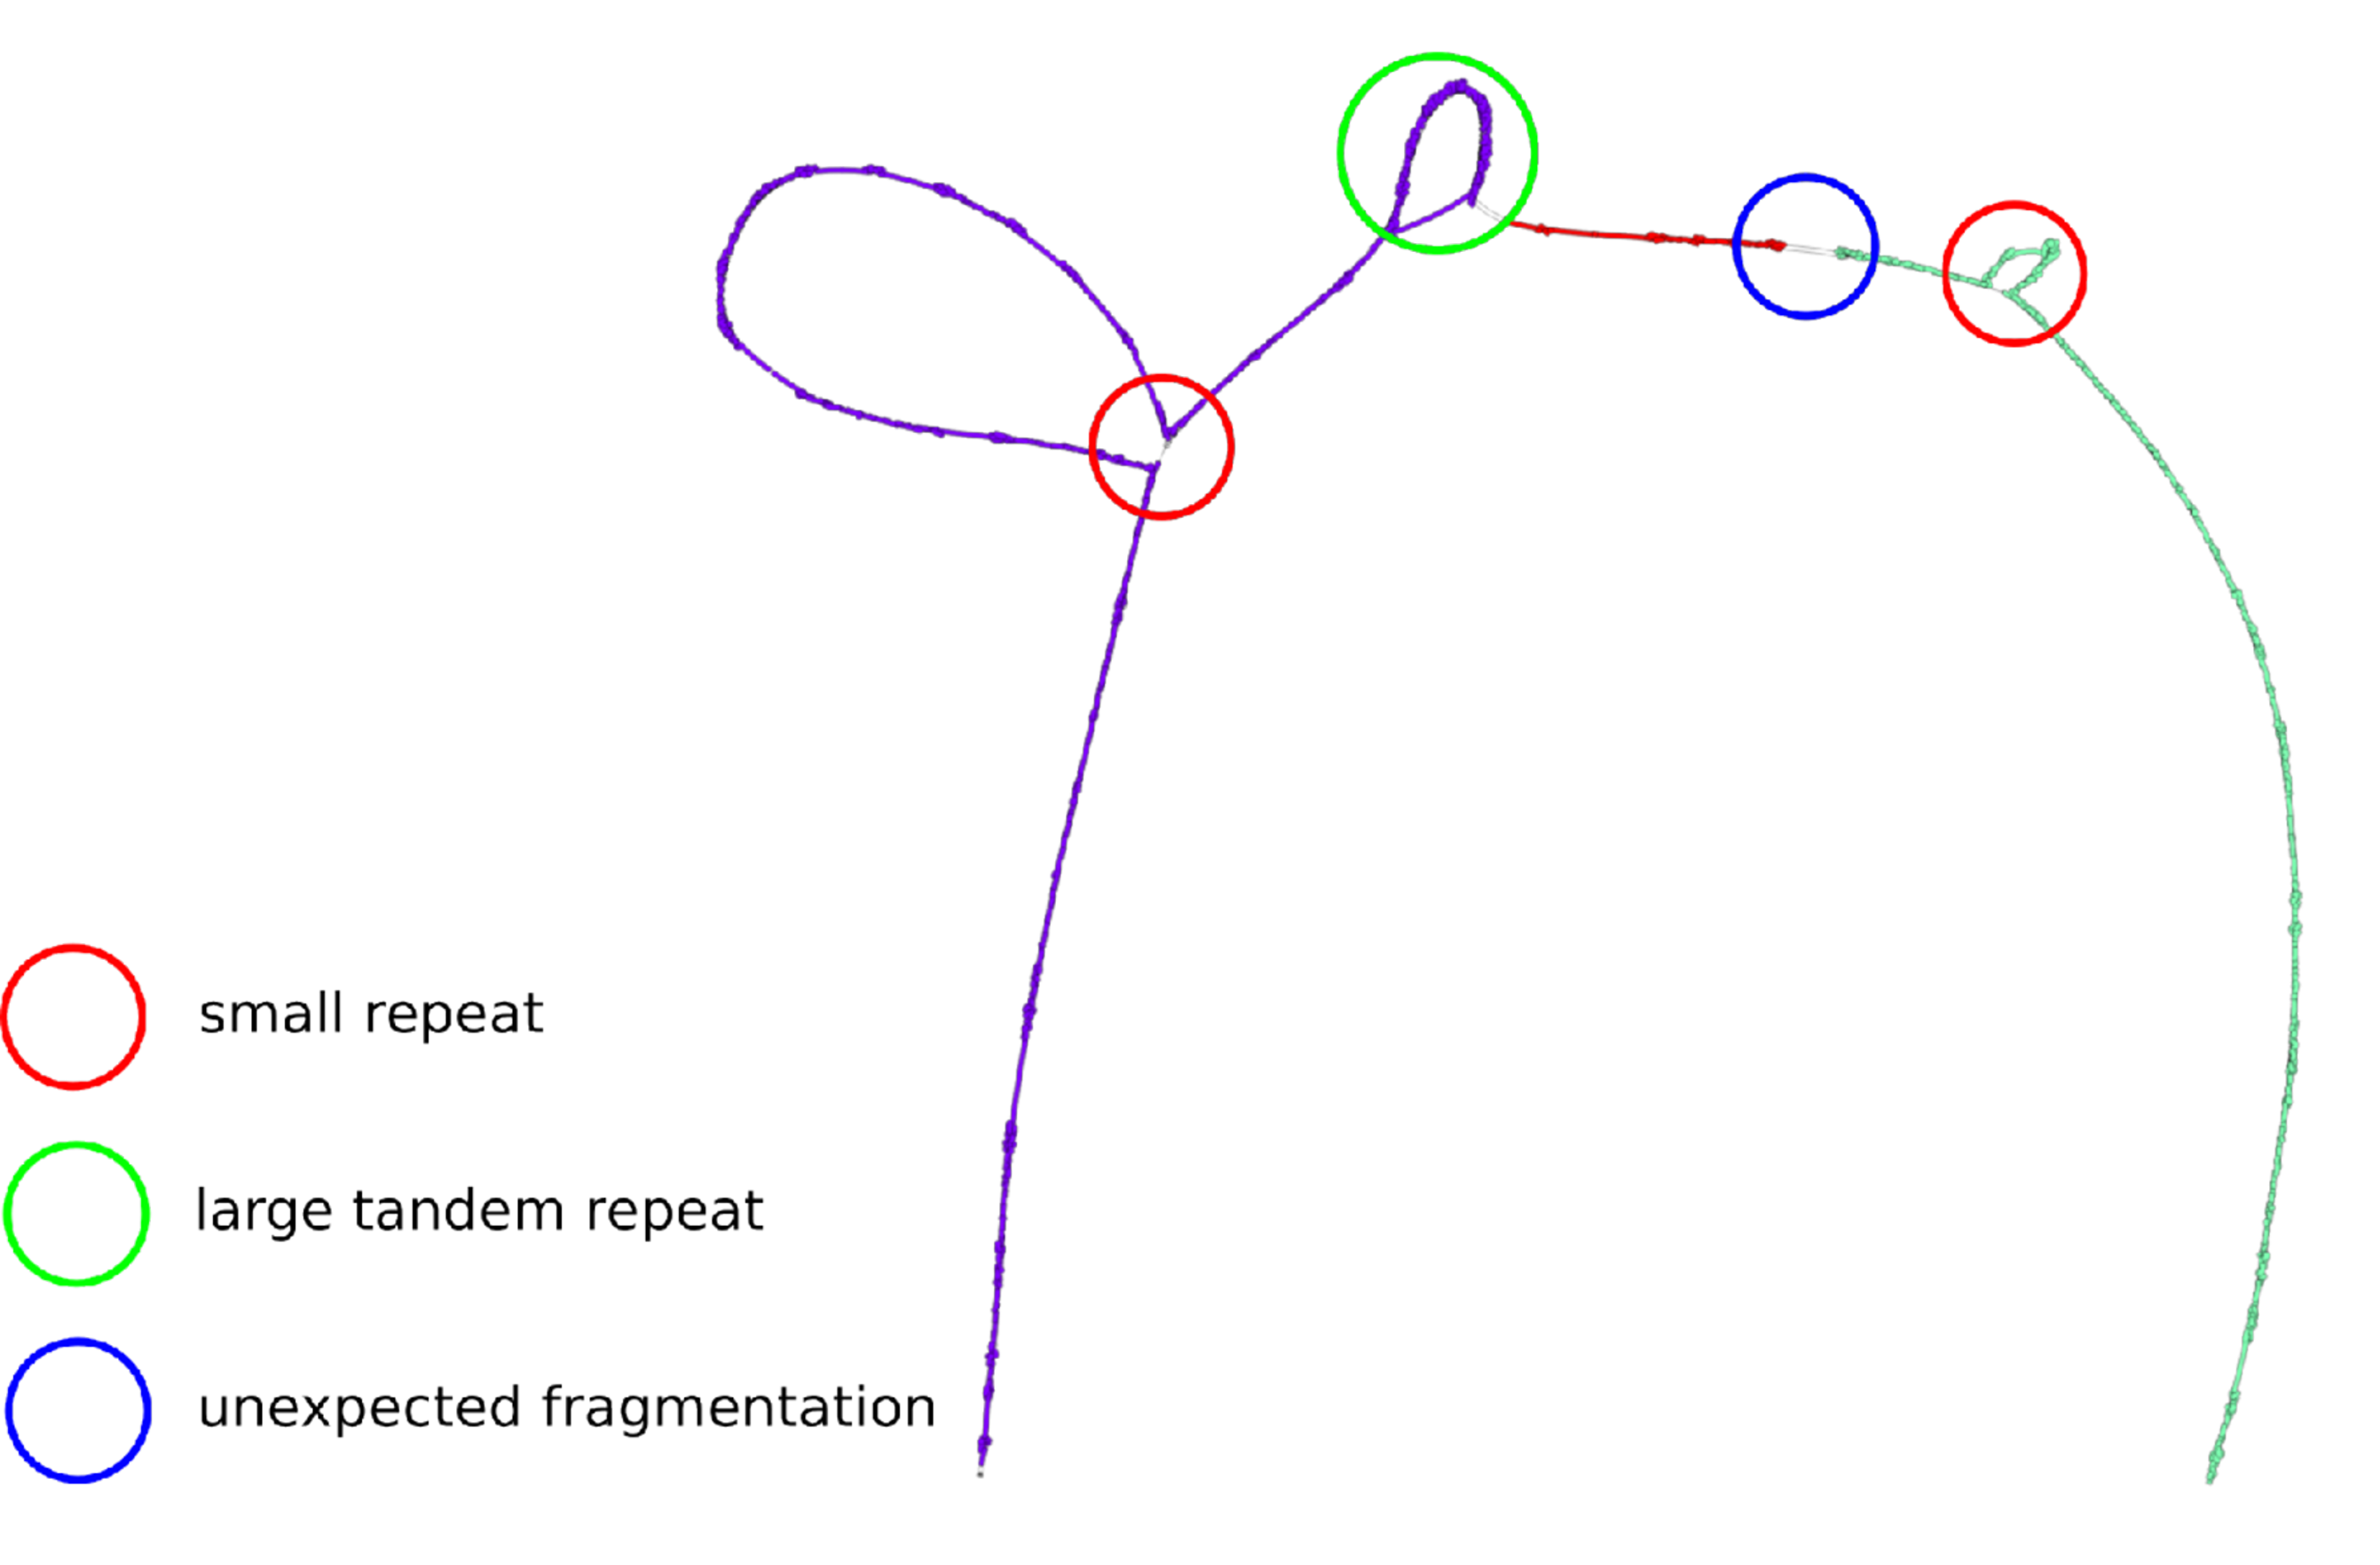
\includegraphics[width=\textwidth]{postassembly/images/t_roseus_projection_annoted.pdf}
    \caption{This graph was the overlap graph (found by \minimap), read used by \canu to build a contigs was are colored with same color. We can observe 2 fragmentation point, one can be explain by a repetition, green circle, we can observe repetition solved by assembly tools, but the fragmentation between green and red can't be explain by a repetition.}
    \label{postassembly:fig:t_roseus_example}
\end{figure}



\subfile{paper/knot.tex}
%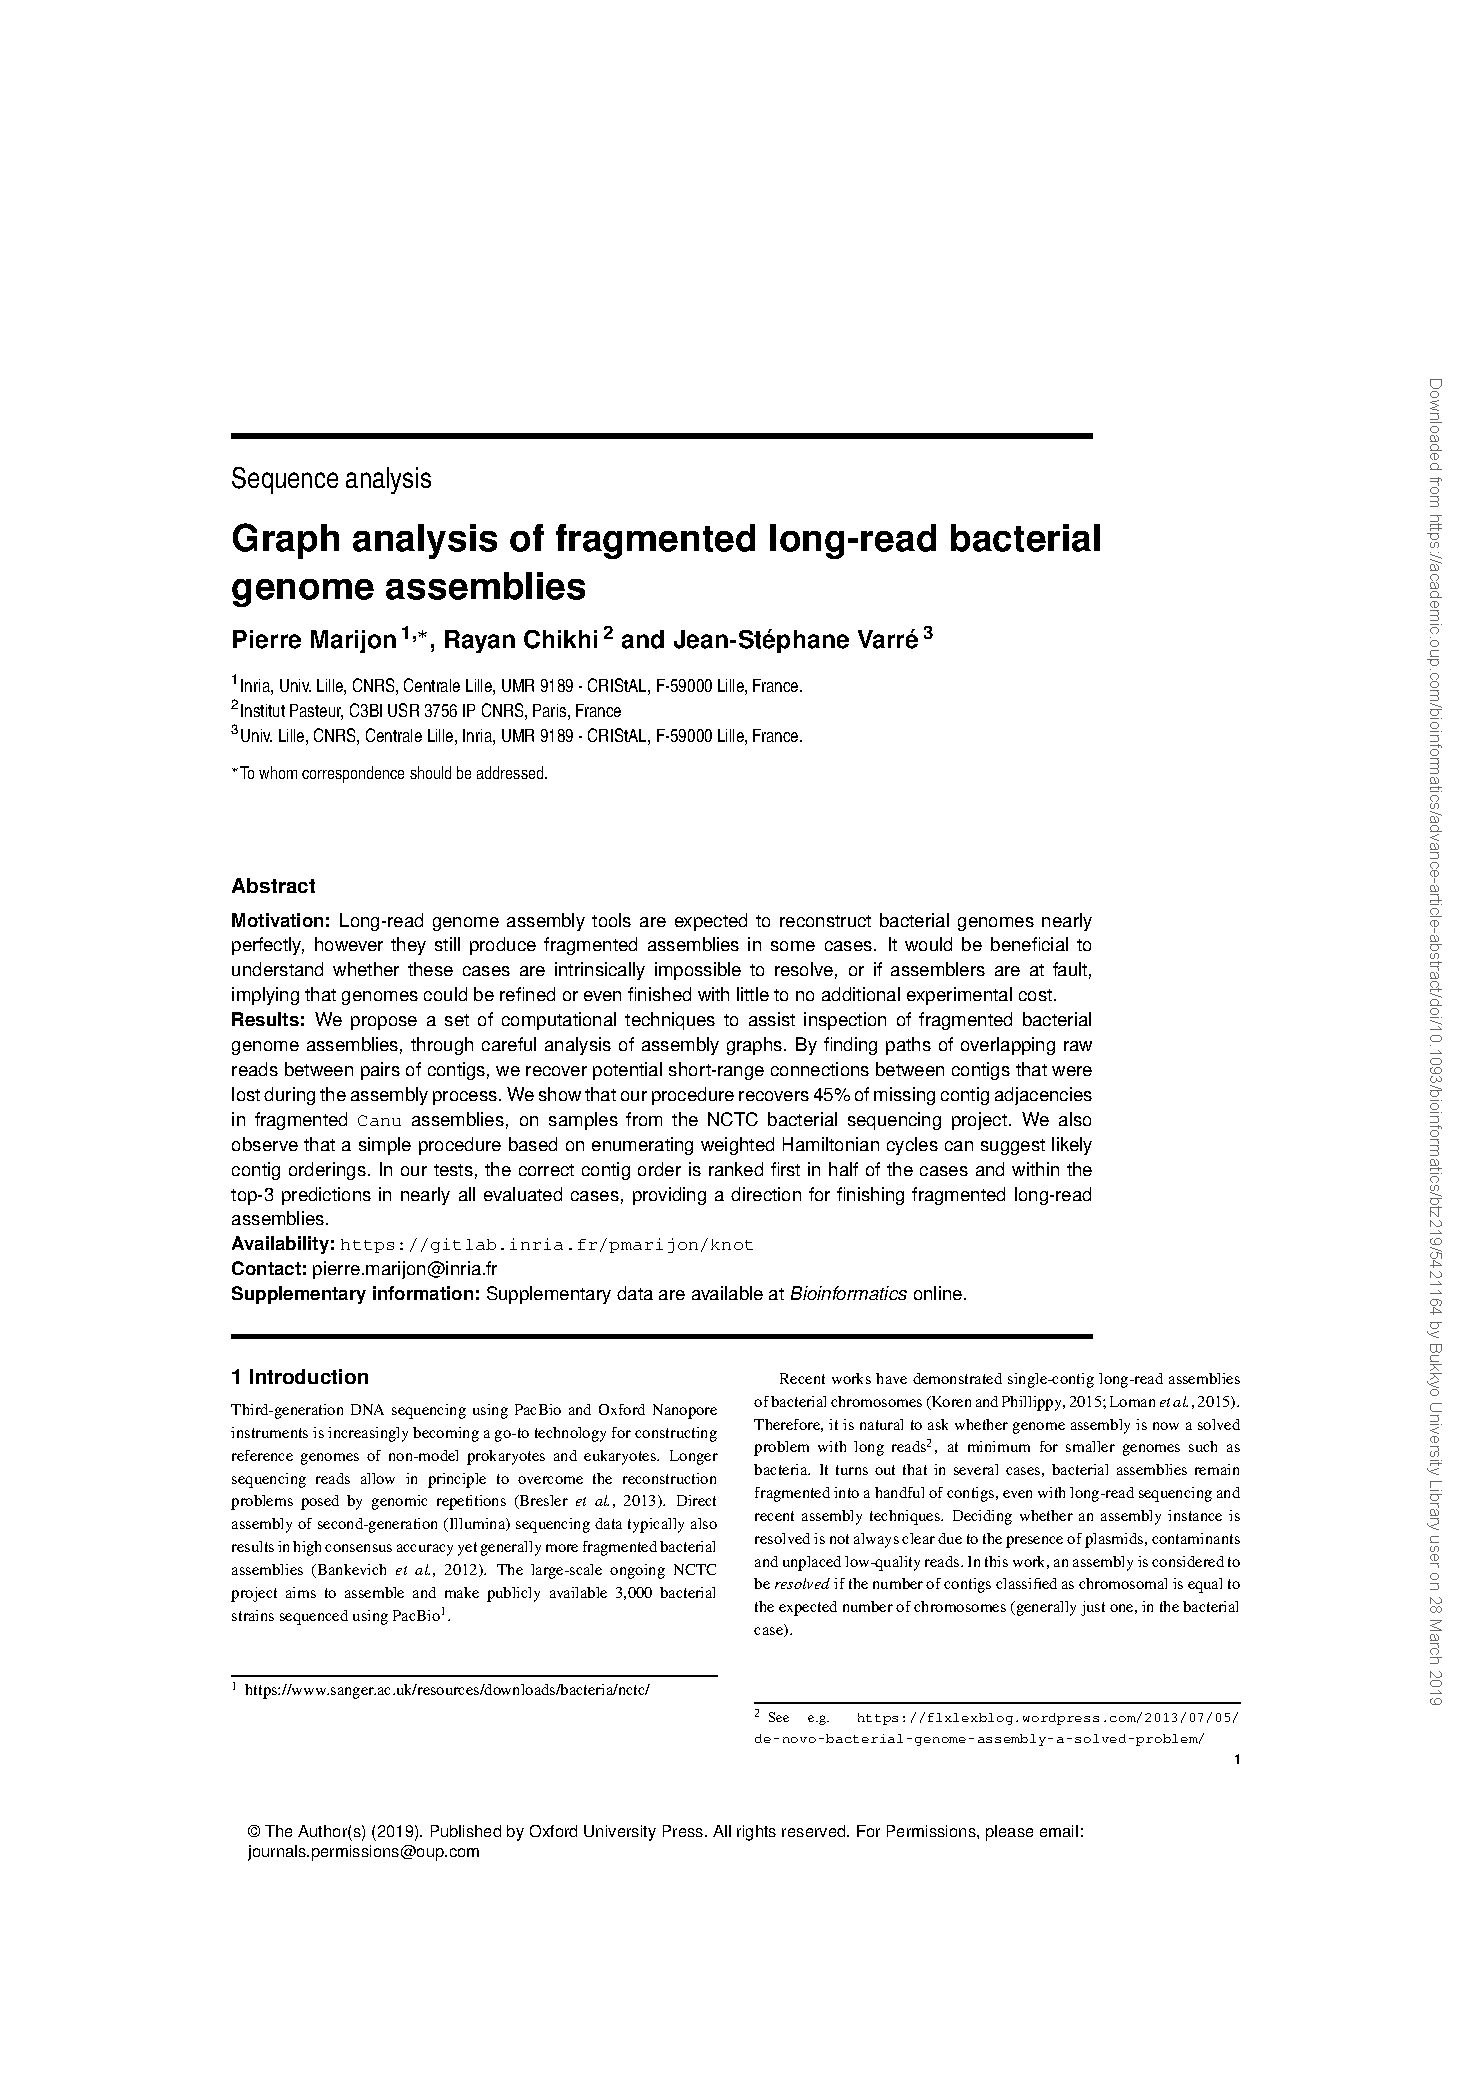
\includepdf[pages=-]{paper/knot.pdf}



\onlyinsubfile{
\bibliographystyle{plainnat}
\bibliography{main}
\addcontentsline{toc}{chapter}{Bibliography}
}

\end{document}